\textbf{Drehbuch}
\begin{enumerate}
\item Kap. 1 - Kap. 5 vom Buch „Die nicht zu kurze Kurzeinführung in MATLAB“ selbstständig durcharbeiten.
\item Die ausgewiesenen Kurzübungen sind abzugeben.
\end{enumerate}
\textbf{Lernziele}
Die Studierenden...
\begin{enumerate}
\item lernen autodidaktisch den Einstig in Matlab.
\item wissen, wie man die Hilfe zu einer Funktion findet.
\item kennen das Command Window.
\item verstehen den Hauptunterschied zwischen einer normalen Variable und einer Matrix.
\item können einfache grafische Darstellungen erstellen.
\end{enumerate}
\section{M2a) übung zu Kapitel 3}
\begin{enumerate}[$(a)$]
\item Studieren Sie die Befehle linspace und logspace. Wo sind die Unterschiede?
\\\\
$\Longrightarrow$ {\color{magenta}\texttt{linspace(xstart, xend)}} erzeugt einen Vektor zwischen \texttt{xstart} und \texttt{xend}, der in 99 gleihe Intervalle unterteilt wird. Der Vektor besteht somit aus 100 linear, gleichmässig verteilten Punkten.
\\
$\Longrightarrow$ {\color{magenta}\texttt{linspace(xstart, xend, n)}} erzeugt einen Vektor zwischen \texttt{xstart} und \texttt{xend}. Der Vektor besteht somit aus \texttt{n} linear, gleichmässig verteilten Punkten.
\begin{itemize}
\item If \texttt{n} is 1, linspace returns \texttt{xend}.
\item If \texttt{n} is zero or negative, linspace returns an empty 1-by-0 matrix.
\item If \texttt{n} is not an integer, linspace rounds down and returns \texttt{floor(n)} points.
\end{itemize}
$\Longrightarrow$ {\color{magenta}\texttt{logspace(xstart, xend)}} erzeugt einen Vektor. Der Vektor besteht somit aus 50 logarithmischen verteilten Punkten zwischen $10^{\texttt{xstart}}$ und $10^{\texttt{xend}}$.
\\
$\Longrightarrow$ {\color{magenta}\texttt{logspace(xstart, xend, n)}} erzeugt \texttt{n} Punkte zwischen $10^{\texttt{xstart}}$ und $10^{\texttt{xend}}$
\\
$\Longrightarrow$ {\color{magenta}\texttt{logspace(xstart, pi, n)}} erzeugt \texttt{n} Punkte zwischen $10^{\texttt{xstart}}$ und $\texttt{pi}$.
\begin{itemize}
\item If \texttt{n} is 1, logspace returns $10^{\texttt{xend}}$.
\item If \texttt{n} is zero or negative, logspace returns an empty row vector.
\item If \texttt{n} is not an integer, logspace rounds \texttt{n} down and returns \texttt{floor(n)} points.
\end{itemize}
\item Erstellen Sie einen Vektor a mit 20 Elementen von 0 bis 19 (ohne linspace).
\\\\
$\Longrightarrow$ {\color{magenta}\texttt{a=(0:1:19)}} oder {\color{magenta}\texttt{a=[0:1:19]}}
\item Erstellen Sie einen Vektor b mit 20 Elementen von 0 bis 2pi.
\\\\
$\Longrightarrow$ {\color{magenta}\texttt{b=linspace(0,2*pi,20)}} \texttt{\%include 2*pi}
\item Erstellen Sie eine 2x20 Matrix A mit den Vektoren a und b.
\\\\
$\Longrightarrow$ {\color{magenta}\texttt{A=[a;b]}}
\item Setzen Sie die beiden Elemente in der letzten Spalte auf 0.
\\\\
$\Longrightarrow$ {\color{magenta}\texttt{A(1,20)=0}}
\\
$\Longrightarrow$ {\color{magenta}\texttt{A(2,20)=0}}
\end{enumerate}
\section{M2b-c) übung zu Kapitel 4 und 5}
\begin{enumerate}[a)]
\item Stellen Sie \texttt{sin(x)}, \texttt{sin(2x)} und \texttt{sin(3x)} gemeinsam in einer Figur dar. Beschriften Sie diese Figur ausführlich (Achsen) und erstellen Sie eine Legende.
\lstinputlisting[language= Matlab, caption={übung M2b) Teil 1}]{../../PROJEKTE/ubungm2a/ubungm2a.m}
\begin{center}
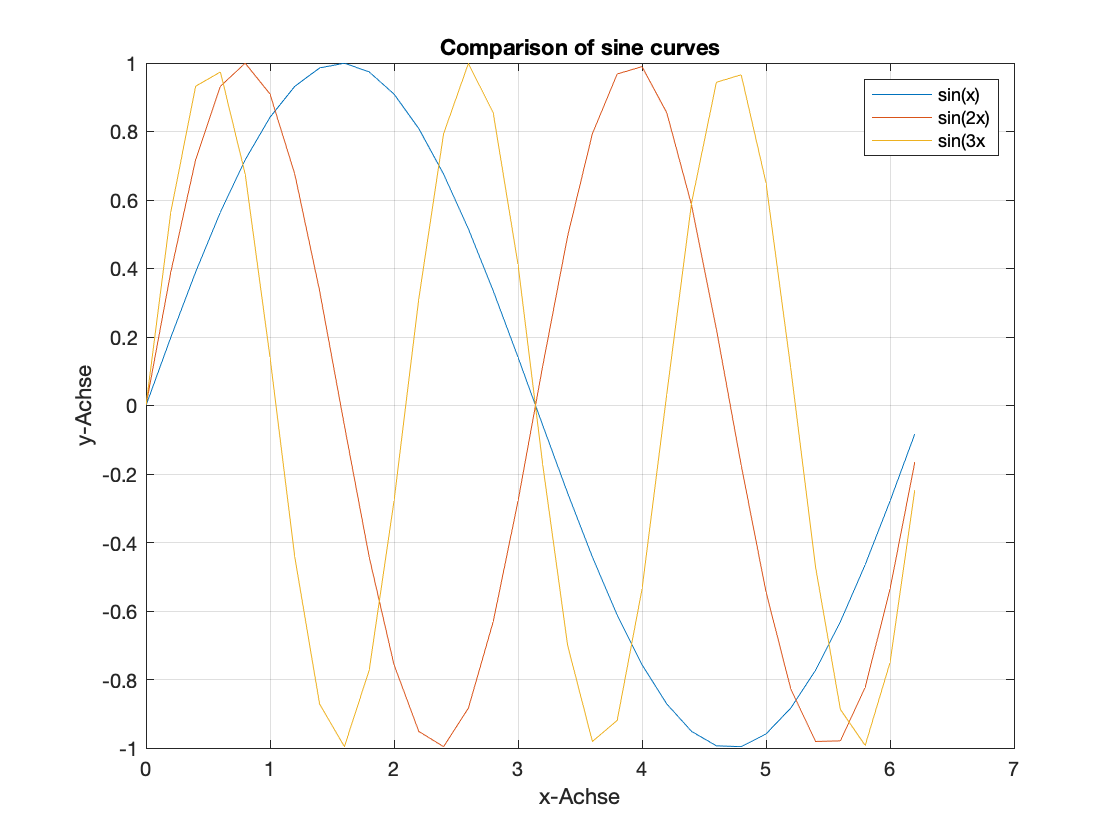
\includegraphics[scale=0.3]{../../PROJEKTE/ubungm2a/ubungm2a.png}
\end{center}
\item Stellen Sie diese Funktionen in einer neün Figure alle untereinander dar.
\lstinputlisting[language=Matlab, caption={übung M2b) Teil 2}]{../../PROJEKTE/ubungm2b/ubungm2b.m}
\begin{center}
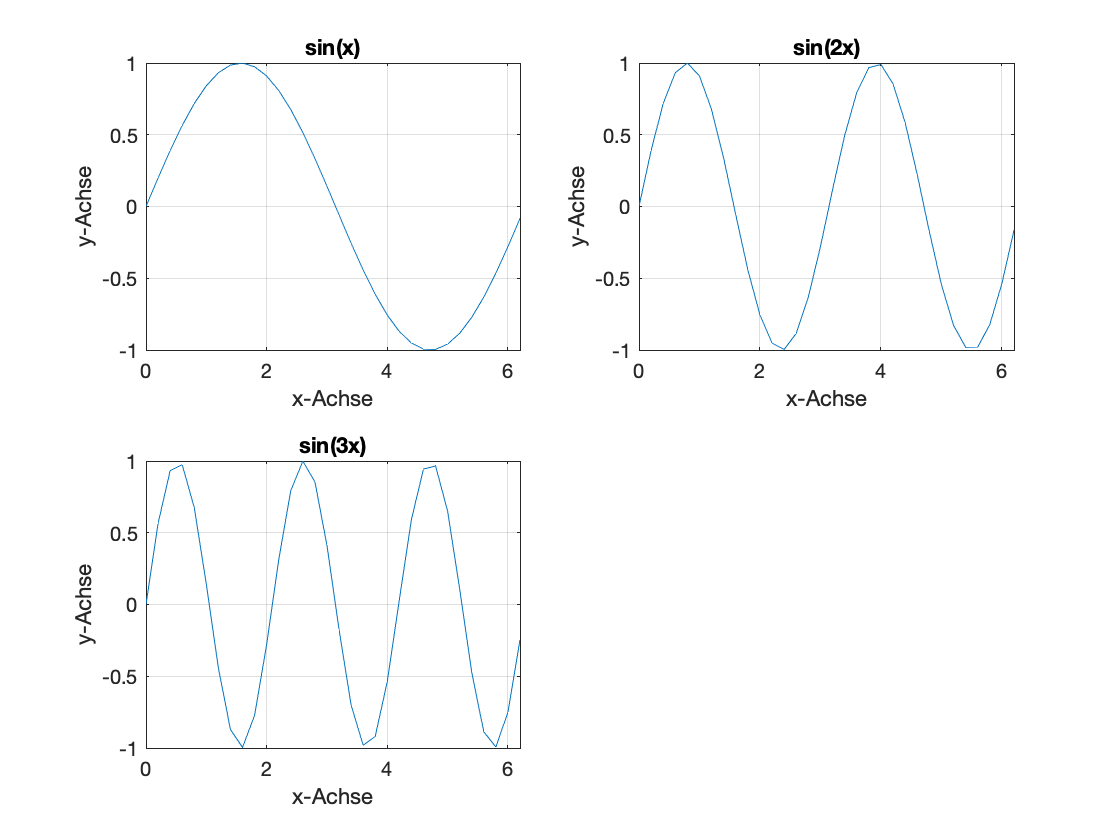
\includegraphics[scale=0.3]{../../PROJEKTE/ubungm2b/ubungm2b.png}
\end{center}
\item Stellen Sie $\texttt{e}^\texttt{x}$ und \texttt{ln(x)} in einer neün Figur dar.
\lstinputlisting[language=Matlab, caption={übung M2b) Teil 3}]{../../PROJEKTE/ubungm2c/ubungm2c.m}
\begin{center}
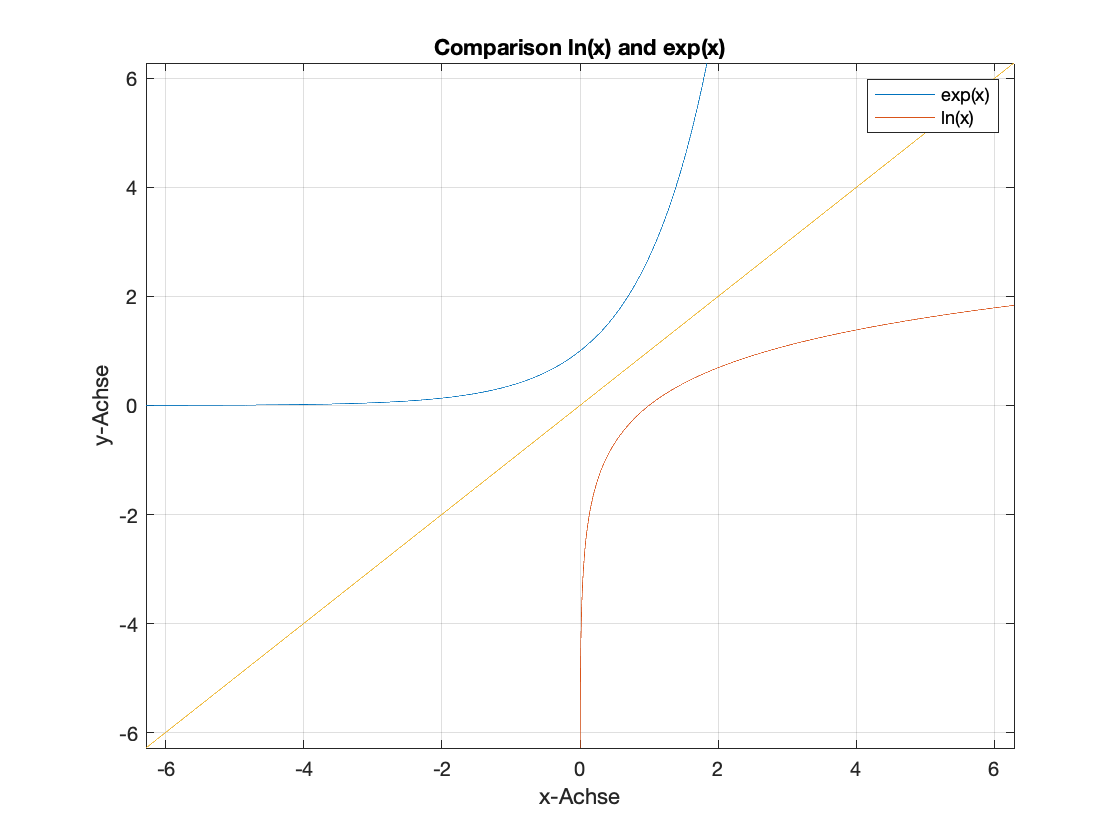
\includegraphics[scale=0.3]{../../PROJEKTE/ubungm2c/ubungm2c.png}
\end{center}
\end{enumerate}










